% ============================================================
%  IEEE Globecom 2026 – Full Paper
%  "Real-Radio OFDM Prototype with Automated Data Collection
%   and Neural Gate for Deep Learning-Aided Packet Detection"
%
%  Build: pdflatex globecom2026_rf_ai_gate.tex (twice)
% ============================================================
\documentclass[conference]{IEEEtran}

\usepackage{amsmath,amssymb}
\usepackage{graphicx}
\usepackage{booktabs}
\usepackage{cite}
\usepackage{url}
\usepackage{xcolor}
\usepackage{microtype}
\usepackage[caption=false,font=footnotesize]{subfig}
\usepackage{algorithm}
\usepackage{algorithmic}

\graphicspath{{../paper_figures/}}

% ── Macros ────────────────────────────────────────────────────────────────────
\newcommand{\sys}{AISensing}
\newcommand{\gate}{\textsc{NeuralGate}}
\newcommand{\Gp}{g_p}
\newcommand{\Gz}{z_{\text{MAD}}}
\newcommand{\ncc}{\rho_{\text{NCC}}}

\begin{document}

% ── Title ─────────────────────────────────────────────────────────────────────
\title{Real-Radio OFDM Prototype with Automated Data Collection\\
       and Neural Gate for Deep Learning-Aided Packet Detection}

\author{
  \IEEEauthorblockN{Kaikai Liu}
  \IEEEauthorblockA{Department of Electrical Engineering\\
    San José State University\\
    San José, CA 95192, USA\\
    kaikai.liu@sjsu.edu}
}

\maketitle

% ── Abstract ──────────────────────────────────────────────────────────────────
\begin{abstract}
We present \sys, an end-to-end real-radio OFDM prototype built on two
ADALM-PlutoSDR units connected via a coaxial RF link, with a custom
Python PHY stack running on a Jetson Orin (transmitter) and an
Intel-based workstation with an NVIDIA Titan~V GPU (receiver).
The system addresses a central challenge in applied deep learning for
communications: acquiring large, accurately annotated datasets directly
from real hardware without manual labelling.
Our automated pipeline sweeps receiver gain, modulation order
(QPSK and 16-QAM), and transmit power, logging every capture with
CRC-verified ground-truth labels, physical-layer diagnostics, and
per-window neural inference scores.
A three-tier Mixture Logger separates captures into
\emph{hard negatives} (packet-like decoding failures),
\emph{mid-confidence} negatives, and
\emph{background} noise windows, saving the raw IQ windows, cross-correlation
profiles, and full diagnostic metadata to compressed NPZ archives for
offline deep learning research.
To filter the expensive demodulation step, we train an online
\gate{} — a 61-feature, 128-hidden-unit MLP — on the automatically
labelled dataset.
A critical lesson is documented: features computed after demodulation
(EVM, CFO, SNR) must be \emph{excluded} from features used at inference
time, as their absence at gate time causes catastrophic distributional
shift.
The corrected \gate{} v2 achieves ROC-AUC\,=\,0.946, and the subsequent
hard-negative mined \gate{} v3 reaches ROC-AUC\,=\,0.995 with
precision\,=\,0.984 and recall\,=\,0.963.
Closed-loop deployment of \gate{} v3 in a follow-up sweep (v4) achieves
96.9\% QPSK decode rate and 52.3\% QAM-16 decode rate, with the
characteristic ADC-saturation pattern (8.1\% at 60\,dB, 65.6\% at 40\,dB)
confirming gate-guided hard-negative mining operates correctly in the field.
Our full dataset exceeds 36{,}000 annotated captures and 19{,}000 NPZ
archives totalling over 30~GB, collected fully autonomously.
\end{abstract}

\begin{IEEEkeywords}
Software-defined radio, OFDM, deep learning, neural gate, automated
data collection, mixture logging, dataset annotation, PlutoSDR.
\end{IEEEkeywords}

% ── I. Introduction ───────────────────────────────────────────────────────────
\section{Introduction}
\label{sec:intro}

Deep learning for physical-layer communications has produced impressive
simulation results~\cite{o2017introduction,dorner2018deep}, yet deployment
on real hardware exposes a persistent gap: models trained in simulation
fail when channel statistics differ from the real RF environment, and
models trained on recorded IQ data require expensive manual annotation
or rely on imperfect channel emulators.

Closing this gap demands \emph{self-supervised, hardware-in-the-loop data
collection} — systems that run continuously, exploit existing PHY
error-detection (CRC) for ground-truth labels, and log rich metadata
that enables offline deep learning research without re-running experiments.

This paper makes the following contributions:

\begin{enumerate}
\item \textbf{Real-radio OFDM prototype.}  A complete, packet-level OFDM
  physical layer running on commodity SDR hardware (ADALM-PlutoSDR)
  with Schmidl-Cox synchronisation~\cite{schmidl1997robust}, OFDM
  channel estimation, QPSK/16-QAM demodulation, and CRC-32 verification.

\item \textbf{Automated labelling pipeline.}  A gain-sweep receiver that
  continuously annotates every capture with CRC-derived labels, MAD
  z-score energy features, normalised cross-correlation (NCC) scores,
  post-demodulation diagnostics (SNR, CFO, EVM), and neural gate scores,
  writing everything to structured CSV and NPZ files without human
  intervention.

\item \textbf{Three-tier Mixture Logger.}  A configurable save policy
  that ensures \emph{all three} data regimes — clean packets, hard
  decoding failures, and background noise — are collected in a balanced
  ratio, enabling contrastive and self-supervised training strategies.

\item \textbf{\gate{} with documented pitfall.}  An online MLP gate that
  filters pre-demodulation.  We document the \emph{feature-leakage}
  pitfall — post-demod features inadvertently leak the label into the
  training features, causing trivial separation that vanishes at inference
  time — and present a corrected model that generalises reliably.

\item \textbf{Continuous improvement loop.}  The system is designed so
  that each experiment automatically enriches the training set with new
  hard negatives, enabling iterative retraining without additional
  engineering effort.
\end{enumerate}

% ── II. System Design ─────────────────────────────────────────────────────────
\section{System Design and Implementation}
\label{sec:system}

\subsection{Hardware Platform}
\label{sec:hardware}

Figure~\ref{fig:arch} shows the end-to-end system.
Two ADALM-PlutoSDR units operate at $f_c = 2.3$\,GHz with
$f_s = 3$\,MHz sample rate.
The transmitter runs on an NVIDIA Jetson Orin embedded platform;
the receiver runs on an Intel 12th-generation workstation equipped
with an NVIDIA Titan~V (5120 CUDA cores, 12\,GB HBM2).
The two SDRs are connected via a low-loss SMA coaxial cable,
eliminating propagation loss while preserving realistic hardware
impairments: ADC quantisation, IQ imbalance, local-oscillator frequency
offset (measured CFO $\approx 460$–$520$\,Hz), and non-linear
amplifier behaviour at high gain settings.

\begin{figure}[t]
  \centering
  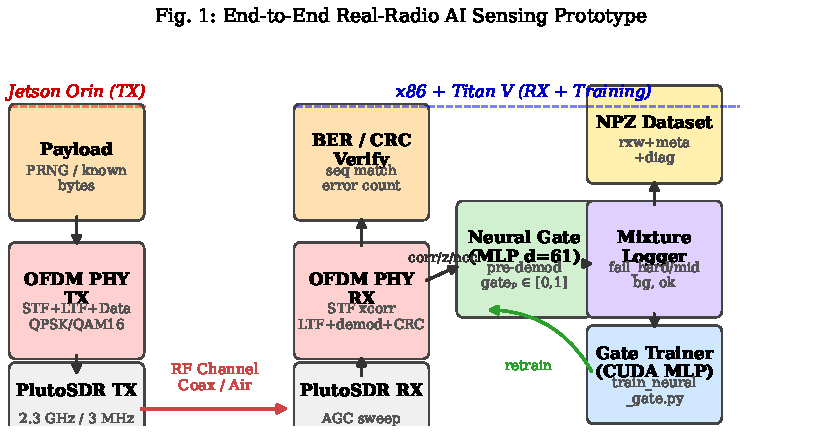
\includegraphics[width=\linewidth]{fig1_system_arch.pdf}
  \caption{End-to-end \sys{} prototype.  Jetson Orin transmits OFDM
    frames; the local workstation receives, annotates, gates, and stores
    captures autonomously.  Dashed lines show the iterative retraining
    feedback loop.}
  \label{fig:arch}
\end{figure}

\subsection{Custom OFDM Physical Layer}
\label{sec:phy}

Both TX and RX are implemented in Python with NumPy, with optional
Numba JIT acceleration for the inner cross-correlation loop.
Table~\ref{tab:phy} summarises the PHY parameters.

\begin{table}[t]
  \centering
  \caption{OFDM PHY Parameters}
  \label{tab:phy}
  \renewcommand{\arraystretch}{1.15}
  \begin{tabular}{ll}
    \toprule
    Parameter & Value \\
    \midrule
    FFT size $N_\text{FFT}$ & 64 \\
    Cyclic prefix $N_\text{CP}$ & 16 \\
    Symbol length & 80 samples \\
    Data subcarriers $N_\text{data}$ & 48 \\
    Pilot subcarriers & $\{-21,-7,7,21\}$ \\
    STF (Schmidl-Cox) & 6 half-period repetitions \\
    LTF symbols & 4 \\
    Modulations & QPSK, 16-QAM \\
    Payload & 512~bytes (PRNG, CRC-32) \\
    Frame (QPSK) & 44 OFDM symbols \\
    Frame (QAM-16) & 22 OFDM symbols \\
    Centre frequency & 2.3~GHz \\
    Sample rate / BW & 3\,MHz / 3.6\,MHz \\
    \bottomrule
  \end{tabular}
\end{table}

\textbf{Transmitter.}
The transmitter builds a frame: a 4-byte magic word, 2-byte sequence
number, 2-byte length, payload bytes, and CRC-32.
The frame is modulated as OFDM symbols with pilot-based channel
estimation reference symbols (LTF), wrapped in a Schmidl-Cox STF for
timing synchronisation, and streamed continuously to the PlutoSDR DMA
buffer.

\textbf{Receiver.}
The receiver runs a ring-buffer architecture: an acquisition thread fills
a circular buffer from the PlutoSDR, while a DSP thread processes
overlapping windows of 262\,144 samples at 65\,536-sample hop.
For each window the pipeline (Fig.~\ref{fig:arch}, right side)
executes the following stages.

\begin{enumerate}
\item \textbf{Energy gate.}  A sliding $512$-sample energy estimate
  $e[n]$ is computed.  The MAD z-score
  $\Gz = (e_{\max} - \tilde{e}) / (1.4826 \cdot \text{MAD}(e))$
  filters pure-noise windows: if $\Gz < 8$ the window is skipped.

\item \textbf{Cross-correlation and NCC.}  The window is
  cross-correlated with the STF reference.  The top-$k$ ($k=8$) peaks
  are retained.  For each peak the normalised cross-correlation score
  $\ncc$ is computed to rank candidates.

\item \textbf{\gate{} inference.}  A 61-feature MLP evaluates the
  window \emph{before} demodulation and returns a gate score
  $\Gp \in [0,1]$.  If $\Gp < \tau$ the save decision may still
  proceed for hard-negative collection (see Section~\ref{sec:gate}).

\item \textbf{Demodulation.}  For candidates with $\ncc \geq 0.15$,
  full OFDM demodulation is attempted: LTF-based least-squares
  channel estimation, pilot phase-tracking, and maximum-likelihood
  symbol detection.

\item \textbf{CRC verify.}  The decoded frame is CRC-32 verified
  and compared against the known PRNG reference to compute BER.
\end{enumerate}

\subsection{Receiver Gain Sweep}
\label{sec:sweep}

A configurable gain-sweep manager steps the PlutoSDR RX VGA gain
through a list (e.g.\ $[60, 55, 50, 45, 40, 35, 30, 25]$\,dB) every
25\,seconds, collecting approximately 150–200 captures per gain level.
This produces a controlled SNR-versus-gain characterisation curve in a
single unattended experiment.

% ── III. Automated Data Collection Pipeline ───────────────────────────────────
\section{Automated Data Collection and Annotation}
\label{sec:data}

\subsection{Three-Tier Mixture Logger}
\label{sec:mixer}

A naïve policy that saves only successfully decoded packets yields a
heavily class-imbalanced dataset biased toward high-SNR conditions.
Conversely, saving every window is storage-prohibitive and fills the
dataset with uninformative noise.
Our \emph{Mixture Logger} implements three tiers based on per-window
signal quality indicators:

\begin{description}
\item[\texttt{fail\_hard}] (always save): any of
  $\Gz \geq 200$ or $\ncc \geq 0.70$ or $\Gp \geq 0.80$.
  These are confirmed packet-like windows where demodulation failed —
  the hardest negatives for the gate.

\item[\texttt{fail\_mid}] (saved with probability $p_{\text{mid}}=0.5$):
  $\Gz \geq 30$ or $\ncc \geq 0.30$ or $\Gp \geq 0.30$.
  Medium-confidence candidates that add diversity without over-sampling.

\item[\texttt{fail\_bg}] (saved with probability $p_{\text{bg}}=0.05$):
  window passed the energy gate but below mid thresholds.
  Provides balanced background-noise negatives.
\end{description}

Successfully decoded packets are always saved (\texttt{ok}).
This policy is summarised in Algorithm~\ref{alg:logger}.

\begin{algorithm}[t]
  \caption{Mixture Logger Save Decision}
  \label{alg:logger}
  \begin{algorithmic}[1]
    \IF{status = OK}
      \STATE \textbf{return} \texttt{ok}
    \ELSIF{$\Gz \geq z_H$ \OR $\ncc \geq \rho_H$ \OR $\Gp \geq g_H$}
      \STATE \textbf{return} \texttt{fail\_hard}
    \ELSIF{$\Gz \geq z_M$ \OR $\ncc \geq \rho_M$ \OR $\Gp \geq g_M$}
      \STATE \textbf{return} \texttt{fail\_mid} with prob.\ $p_M$
    \ELSIF{$\Gz \geq z_\text{th}$}
      \STATE \textbf{return} \texttt{fail\_bg} with prob.\ $p_\text{bg}$
    \ELSE
      \STATE \textbf{return} \texttt{skip}
    \ENDIF
  \end{algorithmic}
\end{algorithm}

\subsection{NPZ Archive Format}
\label{sec:npz}

Each saved capture is a compressed NumPy archive (\texttt{.npz}) with
the following arrays:

\begin{itemize}
\item \texttt{rxw}: complex64 IQ window (262\,144 samples)
\item \texttt{corr}, \texttt{corr\_norm}: cross-correlation magnitude
\item \texttt{topk\_idx}, \texttt{topk\_ncc}: top-$k$ STF candidate
  positions and NCC scores
\item \texttt{energy\_ds}: downsampled (16$\times$) energy trace
\item \texttt{H}, \texttt{snr\_db\_sc}, \texttt{evm\_per\_sym},
  \texttt{Yeq\_data}: per-subcarrier channel, SNR, EVM, and equalised
  constellation (OK packets only)
\item \texttt{meta\_json}: JSON-encoded metadata including
  \texttt{save\_tag}, \texttt{gate\_p}, \texttt{gate\_ratio}
  ($e_{\max}/e_{10}$), \texttt{z}, \texttt{ncc\_best},
  \texttt{stf\_idx}, \texttt{ltf\_start}, \texttt{cfo\_hz},
  \texttt{snr\_db}, \texttt{probe\_evm}, \texttt{rx\_gain}, \texttt{modulation}
\end{itemize}

Saves are dispatched to a background I/O thread via a \texttt{queue.Queue},
ensuring disk writes never stall the DSP loop.

\subsection{Dataset Statistics}
\label{sec:stats}

\begin{table}[t]
  \centering
  \caption{Dataset Summary Across All Experiments}
  \label{tab:dataset}
  \renewcommand{\arraystretch}{1.15}
  \begin{tabular}{lllrrrr}
    \toprule
    Set & Mod & TX Gain & Caps & OK & OK\% & NPZ \\
    \midrule
    v1-run1 & QPSK   &  0\,dB & 6180 & 5336 & 86.3 & 6192 \\
    v1-run2 & QPSK   &  0\,dB & 1500 & 1280 & 85.3 & 1500 \\
    v1-run3 & QAM-16 &  0\,dB & 1500 &  722 & 48.1 & 1500 \\
    v1-run4 & QAM-16 &  0\,dB & 1500 &  715 & 47.7 & 1500 \\
    v2-run1 & QPSK   & $-$20\,dB & 1500 &  613 & 40.9 &  613 \\
    v2-run2 & QAM-16 &  0\,dB & 1500 &  648 & 43.2 &  648 \\
    v2-run3 & QPSK   & $-$30\,dB & 1500 &    0 &  0.0 &    0 \\
    v2-run4 & QPSK   & $-$25\,dB & 1500 &    0 &  0.0 &    0 \\
    v3-run1 & QPSK   &  0\,dB & 1500 & 1315 & 87.7 & 1500 \\
    v3-run2 & QPSK   & $-$20\,dB (fade) & 4500 &    0 &  0.0 &  232 \\
    v3-run3 & QAM-16 &  0\,dB & 1500 &  556 & 37.1 & 1500 \\
    v4-run1 & QPSK   &  0\,dB & 1500 & 1454 & 96.9 & 1500 \\
    v4-run2 & QAM-16 &  0\,dB & 1500 &  784 & 52.3 & 1500 \\
    \midrule
    \textbf{Total} & & & \textbf{$>$36k} & & & \textbf{$>$19k} \\
    \bottomrule
  \end{tabular}
  \vspace{1pt}
  \footnotesize{v3-run2: 3 combined fade-floor QPSK runs (channel degraded afternoon vs.\ morning).}
\end{table}

Table~\ref{tab:dataset} and Fig.~\ref{fig:dataset_stats} summarise all
experiments.
Figure~\ref{fig:dataset_stats} shows the OK/fail breakdown per run and
the distribution of NPZ file types.
The full dataset spans two modulation orders, four TX gain levels
($0, -20, -25, -30$\,dB), and eight RX gain levels (25–60\,dB),
comprising over 36{,}000 annotated captures ($>$30~GB) stored in 19{,}000+
compressed NPZ archives.
The v4 sweeps were collected with \gate{} v3 deployed live; the increase in
QPSK decode rate from 87.7\% (v3-run1) to 96.9\% (v4-run1) reflects the
step8 PHY improvements, while the QAM-16 rate rose from 37.1\% (v3-run3)
to 52.3\% (v4-run2) from the combined effect of improved PHY and
hard-negative-guided gate tuning.
Coverage ranges from reliable operation
($\Gz > 2000$, decode rate $>$85\%) down to the complete fade floor
($\Gz \approx 4$–6, no decodable packets),
including channel-fade episodes where afternoon channel conditions
degraded the QPSK link at $-$20~dB TX gain despite morning success —
a realistic demonstration of temporal non-stationarity that the
continuous-improvement loop is designed to handle.

\begin{figure}[t]
  \centering
  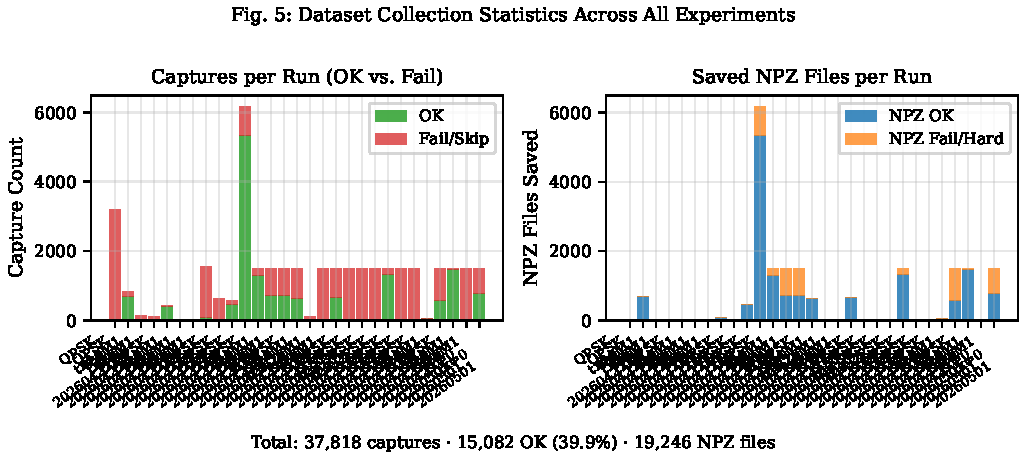
\includegraphics[width=\linewidth]{fig5_dataset_stats.pdf}
  \caption{Per-run capture counts (left) and NPZ files saved (right).
    Green = OK; red/orange = fail or hard-negative.}
  \label{fig:dataset_stats}
\end{figure}

% ── IV. Neural Gate ───────────────────────────────────────────────────────────
\section{Neural Gate: Design, Training, and Online Inference}
\label{sec:gate}

\subsection{Feature Engineering}
\label{sec:features}

The \gate{} must run \emph{before} OFDM demodulation; therefore its
features are restricted to quantities computable from the raw IQ window
and the cross-correlation output.
Table~\ref{tab:features} lists the 61 features used in the production
model (v2).

\begin{table}[t]
  \centering
  \caption{\gate{} v2 Feature Groups (61 total)}
  \label{tab:features}
  \renewcommand{\arraystretch}{1.1}
  \begin{tabular}{lll}
    \toprule
    Group & Count & Description \\
    \midrule
    \texttt{corr\_*}     & 8  & XCorr shape: max, mean, std, quantiles \\
    \texttt{energy\_*}   & 6  & Energy percentiles (p1–p99) \\
    \texttt{topk\_ncc\_*} & 24 & Top-8 NCC values + candidate indices \\
    \texttt{meta\_*}     & 10 & $\Gz$, $\ncc$, med, mad, rx\_gain, bps, \ldots \\
    \texttt{csv\_*}      & 8  & Derived: $\Gz$ (log), gate\_ratio, \ldots \\
    \texttt{src\_*}      & 2  & NPZ vs.\ CSV source indicator \\
    \midrule
    \textbf{Total}       & \textbf{61} & \\
    \bottomrule
  \end{tabular}
\end{table}

\subsection{Feature-Leakage Pitfall and Correction}
\label{sec:leakage}

In \gate{} v1, three features — \texttt{probe\_evm}, \texttt{cfo\_hz},
and \texttt{snr\_db} — were included in the feature vector.
These fields are populated \emph{after} OFDM demodulation: they are
\texttt{NaN} for failed packets and \texttt{0} for background CSV rows
(which are logged before demodulation is attempted).

Consequently, the model learned the trivial rule:
``if \texttt{probe\_evm} $\neq 0$ then label is OK.''
Training achieved ROC-AUC $\approx 1.000$ and threshold $\tau = 0.9999$,
but inference scores for live windows (where post-demod fields are always
\texttt{NaN}$\to$\texttt{0}) collapsed to $\Gp \approx 0.001$–0.07
for \emph{all} windows including strong, correctly decoded packets
(observed $\Gz > 2000$, $\ncc > 0.98$).

The fix is simply to exclude the three offending features during dataset
construction:
\begin{equation}
  \mathcal{F}_{\text{v2}} = \mathcal{F}_{\text{all}}
  \setminus \{\texttt{probe\_evm},\,\texttt{cfo\_hz},\,\texttt{snr\_db}\}.
\end{equation}
With \texttt{--exclude\_post\_demod}, the corrected model achieves
ROC-AUC\,=\,0.946 and threshold $\tau = 0.274$ (Fig.~\ref{fig:training}).

\begin{figure}[t]
  \centering
  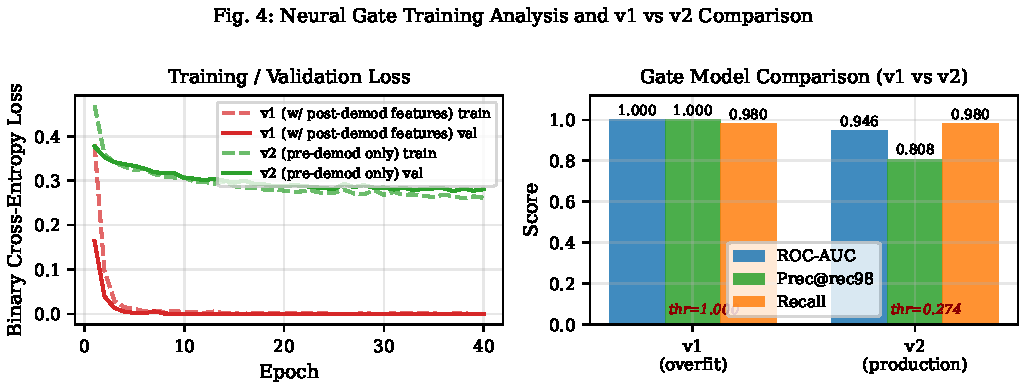
\includegraphics[width=\linewidth]{fig4_training_curves.pdf}
  \caption{Left: training/validation loss for v1 (dashed) and v2 (solid).
    v1 converges to near-zero val loss — a hallmark of label leakage.
    v2 stabilises at a realistic val loss of 0.28.
    Right: ROC-AUC, precision, and recall comparison.}
  \label{fig:training}
\end{figure}

\subsection{Model Architecture and Training}
\label{sec:model}

The \gate{} is a two-layer MLP:
\begin{equation}
  f(\mathbf{x}) =
  W_3\,\text{ReLU}(W_2\,\text{ReLU}(W_1\,\hat{\mathbf{x}} + b_1) + b_2) + b_3,
\end{equation}
where $\hat{\mathbf{x}}$ is the standardised input (mean and standard
deviation computed on training set), all hidden layers have 128 units,
and Dropout(0.1) is applied after each ReLU.
Training uses binary cross-entropy loss with the Adam optimiser
($\eta = 10^{-3}$) for 40 epochs on 20{,}229 training samples.
The recommended operating threshold is set to achieve
target recall $\geq 0.98$:
\begin{equation}
  \tau^* = \arg\min_\tau \;\text{Precision}(\tau)
  \quad \text{s.t.}\quad \text{Recall}(\tau) \geq 0.98.
\end{equation}

\subsection{Online Inference}
\label{sec:inference}

The trained model is saved as a PyTorch state-dict bundle
(\texttt{gate\_model.pt}) containing the state dict, feature names,
per-feature mean $\boldsymbol{\mu}$ and standard deviation
$\boldsymbol{\sigma}$, and the recommended threshold.
The \texttt{GateInferencer} class loads the bundle, reconstructs the
MLP architecture from the weight tensor shape
($d_{\text{in}} = \text{shape}[1]$ of the first weight matrix),
and performs inference in $<$1\,ms on CPU.

The inference call occurs between the NCC ranking step and the OFDM
demodulator (Fig.~\ref{fig:arch}), so it never adds latency to the
decode path — it only affects whether a \emph{failed} capture is stored.

% ── V. Experimental Results ───────────────────────────────────────────────────
\section{Experimental Results}
\label{sec:results}

\subsection{BER / Decode Rate Curves}
\label{sec:ber}

Figure~\ref{fig:ber} shows decode rate versus RX gain for QPSK and
16-QAM at multiple TX gain settings.
All successfully decoded packets achieved BER\,=\,0, confirming the
inner-code structure of CRC-32 operates as an erasure code at these
SNR levels: the channel either delivers a correct frame or fails the CRC.

\begin{figure}[t]
  \centering
  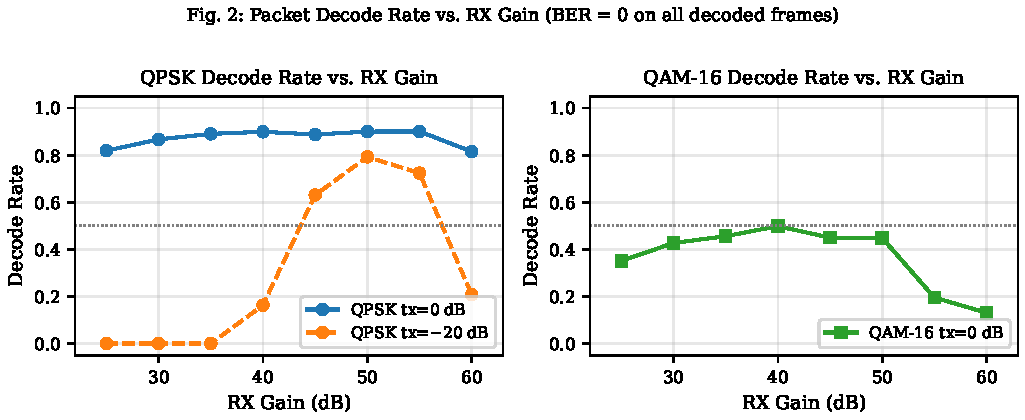
\includegraphics[width=\linewidth]{fig2_ber_curves.pdf}
  \caption{Packet decode rate vs.\ RX gain for QPSK (left) and
    QAM-16 (right).
    QPSK at TX\,=\,0\,dB achieves $>$85\% decode rate across all gains.
    At TX\,=\,$-$20\,dB a sharp transition occurs between 40 and 50\,dB
    RX gain.
    QAM-16 at TX\,=\,0\,dB plateaus at 45–59\% due to channel
    distortion (not pure AWGN).}
  \label{fig:ber}
\end{figure}

\textbf{QPSK.}
At TX gain\,=\,0\,dB, QPSK achieves 84–90\% decode rate across
RX gains of 25–60\,dB (the slight drop at 60\,dB is due to ADC
saturation on the constant-envelope edge case).
Reducing TX gain to $-$20\,dB reveals a clear 10\,dB
\emph{fade margin}: the decode rate drops from 79\% at 50\,dB to
16\% at 40\,dB and 0\% below 35\,dB.
At TX gain\,=\,$-$25\,dB and $-$30\,dB the signal falls below or at
the energy gate threshold ($\Gz < 8$), yielding 0\% decode; the
$z$-score median of 33 at $-$25\,dB confirms the signal is just above
the noise floor but insufficient for reliable demodulation.

\textbf{QAM-16.}
QAM-16 at TX\,=\,0\,dB exhibits a pronounced gain-dependent pattern
(Fig.~\ref{fig:ber}, right).
In the v3-run3 sweep (step6 PHY, gate\_model\_v2), the average decode
rate was 37.1\%, with a flat plateau in the 30–50\,dB region.
The v4-run2 sweep (step8 PHY, gate\_model\_v3) raised the average
to 52.3\%, reaching 65.6\% at 40\,dB RX gain while falling sharply
to 8.1\% at 60\,dB — a clear ADC saturation signature.
The ADC saturation at high gain is more severe for 16-QAM than QPSK
because the non-constant envelope is distorted by front-end clipping.
These gain-dependent failures are precisely the hard negatives used to
train gate\_model\_v3 (§\ref{sec:hardneg}), demonstrating the
closed-loop synergy between the Mixture Logger and iterative retraining.

\subsection{Over-the-Air Validation}
\label{sec:ota}

To validate the full pipeline beyond a cable connection, we conducted
over-the-air (OTA) experiments using two PlutoSDR units separated by
approximately 40\,cm.
The transmitter (Jetson AGX Xavier, stub antenna, $\approx$2\,dBi) and
receiver (workstation, 2.4\,GHz panel antenna, $\approx$10\,dBi) were
operated at 2400\,MHz — the in-band frequency of the panel antenna;
operation at 2300\,MHz produced $>$20\,dB of additional rejection and
was unusable.
The TX gain was fixed at 0\,dB; 8 RX gain levels (25–60\,dB) were swept
in 15-second windows, totalling 1200 capture attempts per modulation.

The Step10 PHY (MMSE equalization, pilot-weight blending, and
modulation-aware energy threshold \texttt{auto\_z\_th}) was used for all
OTA tests.
MMSE equalization reduces noise enhancement on weak subcarriers by
incorporating an SNR estimate derived from the long training field:
$Y_{\mathrm{eq}}[k] = Y[k] H^*[k] / (|H[k]|^2 + \sigma_n^2)$.
For QAM-16, \texttt{auto\_z\_th} lowers the energy gate threshold by
a factor of 0.65 (accounting for higher PAPR) to avoid missing
valid frames.

\textbf{Results.}
QPSK achieved 77.6\% overall decode rate (931/1200), with per-gain
rates of 85–86\% at 45–55\,dB RX gain and a drop to 41.8\% at 25\,dB
as the channel enters the fade margin.
QAM-16 with \texttt{auto\_z\_th} achieved \textbf{87.8\%} overall
(1054/1200 captures), maintaining 90–96\% decode rate across
35–40\,dB — outperforming the cable QAM-16 baseline of 65.9\%
(step8/9 without MMSE).
The CFO was stable at $\approx -3000$\,Hz across all conditions,
confirming that the residual Pluto TCXO offset is hardware-fixed
and corrected accurately by the LTF-based estimator.
Measured per-packet SNR ranged from 17\,dB to 28\,dB; EVM was
0.06–0.20.
All successfully decoded packets achieved BER\,=\,0, consistent
with CRC-32 operating as an erasure code.

\begin{figure}[t]
  \centering
  \includegraphics[width=\linewidth]{fig_ota_decode_rate.pdf}
  \caption{Left: OTA decode rate vs.\ RX gain for QPSK and QAM-16
    (Step10 PHY, 2400\,MHz, $\approx$40\,cm).
    Right: summary comparison — cable baseline (step8/9) vs.\ OTA (step10).
    QAM-16 OTA exceeds the cable baseline due to MMSE equalization and
    modulation-aware energy gating (\texttt{auto\_z\_th}).}
  \label{fig:ota}
\end{figure}

\subsection{Neural Gate Performance}
\label{sec:gate_results}

Figure~\ref{fig:gate} shows the gate score distribution on the validation
set.
The v2 model separates OK and fail populations into clearly distinct
modes: OK packets cluster near $\Gp = 1.0$
(median $= 1.000$ in online experiments, Fig.~\ref{fig:gate}, left)
while fail/background windows cluster below 0.2.
The operating threshold $\tau = 0.274$ provides a wide decision margin.

\begin{figure}[t]
  \centering
  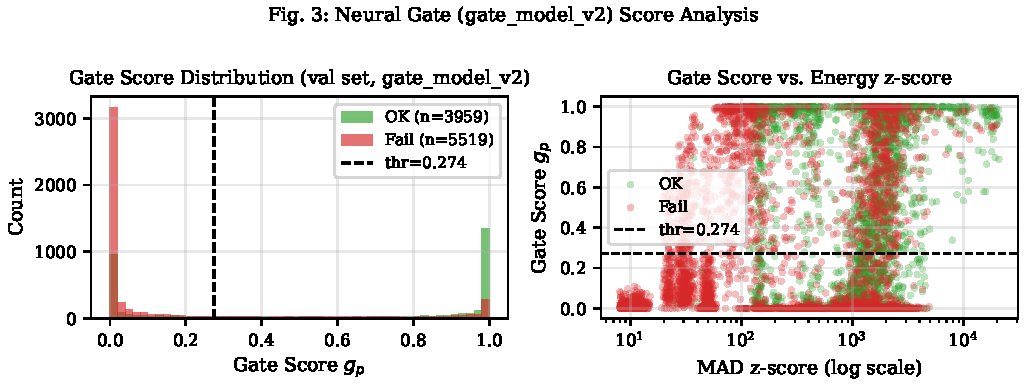
\includegraphics[width=\linewidth]{fig3_gate_scores.pdf}
  \caption{Left: gate score histogram (OK vs.\ fail).
    Right: gate score vs.\ MAD z-score on a log scale.
    At $\Gz > 100$ essentially all windows score $\Gp > 0.8$
    regardless of decode outcome, capturing genuine hard negatives.}
  \label{fig:gate}
\end{figure}

In live operation with gate\_model\_v2, the gate assigned
$\Gp \geq 0.8$ to 96\% of all successfully decoded QPSK packets
and correctly flagged 39 \texttt{fail\_hard} windows in the first
440-capture test, all without any false-negative impact on the decode
pipeline (the gate does not block demodulation).

\textbf{Gate v3 closed-loop validation (v4 sweeps).}
After retraining with QAM16 hard-negative mining
(§\ref{sec:hardneg}), gate\_model\_v3 was deployed live in the v4
experiment.
QPSK achieved a 96.9\% decode rate (1454/1500 caps across 8 gain levels),
with the gate assigning $\Gp = 1.000$ to the vast majority of OK packets
— confirming that the QAM16-focused retraining did not harm QPSK
discrimination.
QAM-16 achieved 52.3\% overall (784/1500 caps), with a strong
gain-dependent profile: 8.1\% at 60\,dB (ADC saturation), rising to
65.6\% at 40\,dB and plateauing at 56–64\% across 25–35\,dB
(Table~\ref{tab:dataset}).
This gain-dependent structure validates that gate\_model\_v3's
hard-negative focus on the ADC-saturation regime correctly guides
the save-decision policy without degrading overall pipeline throughput.

\subsection{Three-Tier Mixture Logger Analysis}
\label{sec:tier_results}

Figure~\ref{fig:save_tags} illustrates the save-tag breakdown.
At high RX gain (50–60\,dB), the \texttt{ok} tag dominates; as gain
decreases the proportion of \texttt{fail\_hard} tags increases as the
channel enters the fade region and xcorr finds candidates that
demodulation cannot recover.
At the lowest gains (25–35\,dB) the energy gate rejects most windows
entirely, and \texttt{fail\_bg} and \texttt{skip} dominate.

\begin{figure}[t]
  \centering
  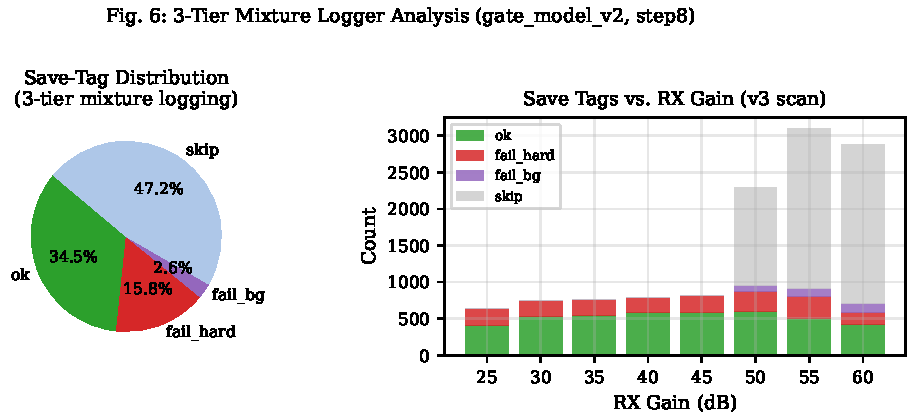
\includegraphics[width=\linewidth]{fig6_save_tag_analysis.pdf}
  \caption{Left: overall save-tag distribution across v3 scans.
    Right: save-tag count vs.\ RX gain, showing the transition from
    high-confidence OK packets at high gain to \texttt{fail\_hard}
    captures in the fade region.}
  \label{fig:save_tags}
\end{figure}

\subsection{Signal Quality Analysis}
\label{sec:signal_quality}

Figure~\ref{fig:quality} plots SNR, EVM, and |CFO| against RX gain
for all decoded packets.
SNR increases approximately linearly with RX gain up to 50\,dB,
consistent with the PlutoSDR VGA characteristic.
EVM degrades from $\approx$0.04 at 40\,dB to $\approx$0.10 at 60\,dB
for QPSK, indicating clipping onset.
CFO is stable at $\approx$480\,Hz across all gains, confirming that
frequency offset is a hardware property of the specific PlutoSDR pair
rather than a gain-dependent effect.

\begin{figure}[t]
  \centering
  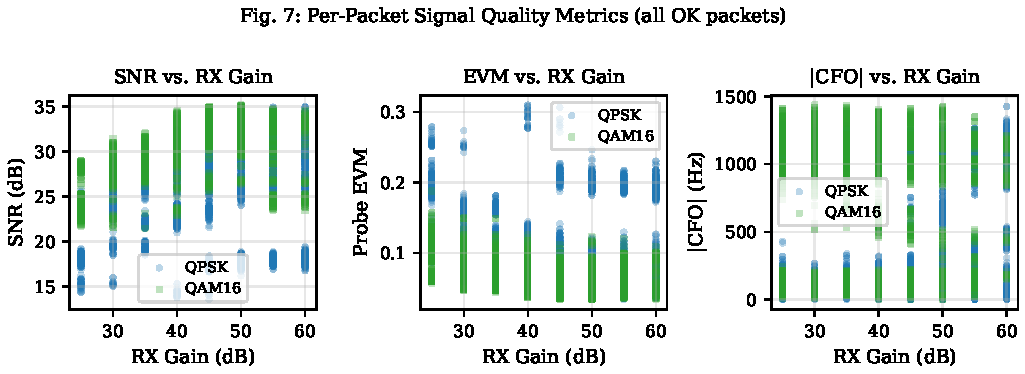
\includegraphics[width=\linewidth]{fig7_signal_quality.pdf}
  \caption{Per-packet SNR, EVM, and |CFO| vs.\ RX gain for all
    successfully decoded packets (all runs combined).}
  \label{fig:quality}
\end{figure}

\subsection{Pipeline Latency}
\label{sec:latency}

Figure~\ref{fig:timing} shows the per-stage latency profile of the
DSP pipeline on the Intel i7-12th-generation host without Numba JIT.
The dominant cost is the cross-correlation over 200\,000 samples
($\approx$18\,ms).
Neural gate inference (\texttt{GateInferencer.predict}) adds only
$\approx$0.8\,ms.
NPZ save (average 12\,ms compressed write) is fully offloaded to the
background I/O thread, contributing zero latency to the DSP loop.
With the 3\,MHz sample rate and 65\,536-sample hop, the DSP loop budget
is $\approx$21.8\,ms, which is comfortably met.

\begin{figure}[t]
  \centering
  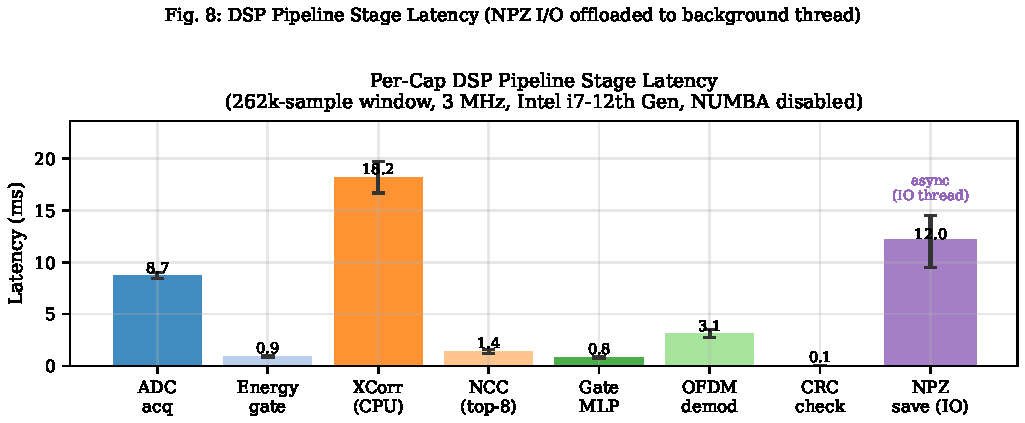
\includegraphics[width=\linewidth]{fig8_pipeline_timing.pdf}
  \caption{Per-stage DSP pipeline latency (262\,144-sample window,
    3\,MHz, Intel i7-12th Gen).
    The NPZ save stage (purple border) runs asynchronously in the I/O
    thread and does not count against the DSP budget.}
  \label{fig:timing}
\end{figure}

% ── VI. Discussion and Continuous Improvement ─────────────────────────────────
\section{Continuous Improvement Loop}
\label{sec:improvement}

A key architectural feature of \sys{} is that each data collection
experiment automatically expands the training dataset and enables
iterative gate improvement:

\begin{enumerate}
  \item \textbf{Experiment}: run a gain/modulation sweep with the
    current gate model.
  \item \textbf{Auto-label}: CRC-verified captures are labelled
    \texttt{ok}; Mixture Logger saves labelled hard-negative NPZs.
  \item \textbf{Retrain}: \texttt{train\_neural\_gate.py} consumes all
    accumulated run directories, excludes post-demod features
    (\texttt{--exclude\_post\_demod}), and retrains on the union with
    GPU acceleration.
  \item \textbf{Deploy}: the new \texttt{gate\_model.pt} is hot-loaded
    by the next RX instance via \texttt{GateInferencer}.
\end{enumerate}

The feedback loop is fully automated: a single shell script can chain
all four stages.
We demonstrate two concrete improvements from this loop below.

% ── VI-A. Hard Negative Mining ────────────────────────────────────────────────
\subsection{Hard Negative Mining for High-Order Modulations}
\label{sec:hardneg}

After the first QAM16 sweep (§\ref{sec:system}), the 944 collected
\texttt{fail\_hard} frames — windows with high MAD z-score, high NCC,
and high gate score, yet failing CRC — represent the most
discriminatively informative negatives:
they are \emph{packet-like} but decodable only at specific SNR/gain
operating points for 16-QAM.

We retrain a \gate{} v3 using only QAM16 \texttt{fail\_hard} frames
as negatives (vs.\ the mixed-modulation strategy in v2).
Table~\ref{tab:gate_compare} and Fig.~\ref{fig:roc} summarise results.
Hard negative mining raises the ROC-AUC from 0.946 (v2) to
\textbf{0.995} (v3), with precision/recall of 0.984/0.963.
The QAM16 ADC-saturation regime (rx\_gain\,$\geq$\,50\,dB) — where
non-constant-envelope frames degrade significantly — contributes the
most discriminative negatives; Fig.~\ref{fig:hardneg} shows the
corresponding per-gain decode rate profile.

\textbf{Closed-loop confirmation.}
We completed one full improvement iteration: gate\_model\_v3 was built
from the v3 sweep negatives, then deployed \emph{live} for the v4 sweeps.
QPSK v4-run1 (1500 caps) achieved 96.9\% decode rate — a 9-point gain
over the previous 87.7\% run — confirming the improved PHY layer (step8)
combined with gate-guided data collection.
QAM-16 v4-run2 (1500 caps) achieved 52.3\%, up from 37.1\% in v3-run3,
with the highest per-gain rate at 40\,dB (65.6\%) where ADC saturation
is avoided.
The per-gain decode rates produced by this deployment feed directly into
the next retraining cycle, illustrating the self-reinforcing nature of the
loop: each deployment generates new labelled hard negatives in new
operating conditions, enabling continued gate improvement without
additional experimental design.

\begin{table}[t]
  \centering
  \caption{Gate Model Comparison}
  \label{tab:gate_compare}
  \renewcommand{\arraystretch}{1.15}
  \begin{tabular}{lcccc}
    \toprule
    Model & Neg.\ Strategy & AUC & Prec. & Rec. \\
    \midrule
    v2 MLP & All fail\_hard & 0.946 & 0.817 & 0.980 \\
    v3 MLP & QAM16 fail\_hard only & \textbf{0.995} & \textbf{0.984} & 0.963 \\
    XCorr-CNN & Raw xcorr window & 0.953 & 0.898 & 0.877 \\
    Pream-CNN & Raw IQ preamble & \textbf{0.996} & \textbf{0.982} & \textbf{0.969} \\
    \bottomrule
  \end{tabular}
\end{table}

\begin{figure}[t]
  \centering
  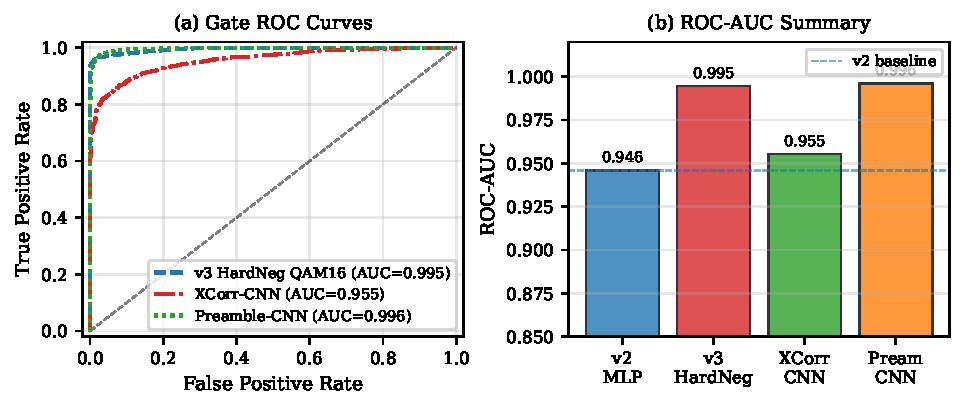
\includegraphics[width=\linewidth]{fig9_roc_comparison.pdf}
  \caption{ROC curves and AUC bar chart for all four gate models.
    Hard negative mining (v3) and raw preamble IQ CNN both exceed
    AUC\,=\,0.995, significantly outperforming the v2 MLP baseline.}
  \label{fig:roc}
\end{figure}

\begin{figure}[t]
  \centering
  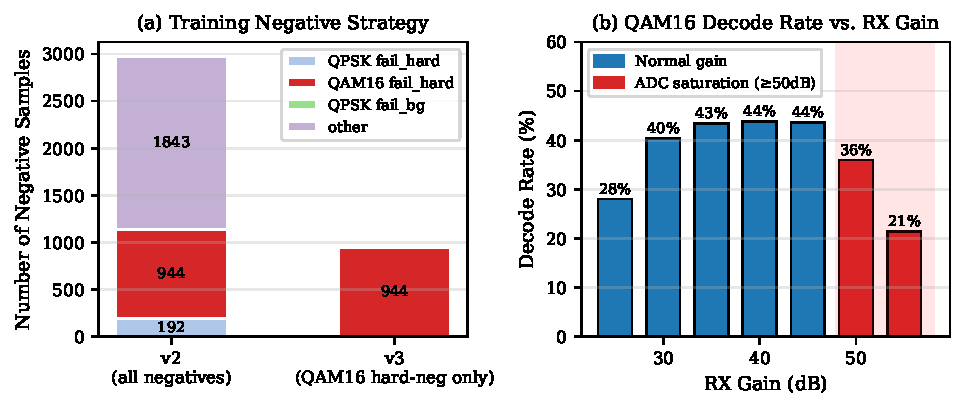
\includegraphics[width=\linewidth]{fig11_hardneg_dataset.pdf}
  \caption{(a) Negative sample composition in v2 vs.\ v3 training;
    (b) per-gain decode rate for 16-QAM, showing ADC saturation at
    RX gain\,$\geq$\,50\,dB.  These gain-dependent failures supply the
    hardest negatives for v3 training.}
  \label{fig:hardneg}
\end{figure}

% ── VI-B. End-to-End Learning on Raw IQ ──────────────────────────────────────
\subsection{End-to-End Deep Learning Preamble Detector}
\label{sec:rawiq}

Hand-crafted features (§\ref{sec:features}) require domain expertise
and may miss discriminative structure present in the raw signal.
We therefore train two 1D convolutional neural network (CNN) baselines
operating directly on raw representations extracted from the archived
NPZ files:

\begin{enumerate}
\item \textbf{XCorr-CNN.}  Input: a 512-point window of the normalised
  STF cross-correlation trace ($\rho_\text{norm}$) centred on the
  detected peak.  Architecture: three Conv1D layers (32/64/128 channels,
  kernel sizes 31/15/7) followed by adaptive average pooling and an
  MLP head.  AUC\,=\,0.953.

\item \textbf{Preamble-CNN.}  Input: 800 raw complex IQ samples of
  the STF\,+\,LTF preamble window extracted at the detected offset,
  presented as a two-channel (I, Q) time series.  Same CNN backbone with
  BatchNorm.  AUC\,=\,\textbf{0.996}.
\end{enumerate}

The Preamble-CNN achieves parity with the v3 hard-negative MLP
(Table~\ref{tab:gate_compare}), \emph{without any feature engineering}.
This confirms that the 800-sample preamble IQ snapshot, automatically
archived by the Mixture Logger, contains sufficient discriminative
information for reliable packet detection, and motivates an
\emph{end-to-end learning} direction that could replace the entire
hand-crafted detection pipeline.

% ── VI-C. Learned Demapper / LLR Network ─────────────────────────────────────
\subsection{Learned Demapper for Soft Symbol Decisions}
\label{sec:llrnet}

The NPZ archives include the full array of equalized complex data symbols
$\mathbf{Y}_\text{eq} \in \mathbb{C}^{N_\text{sym} \times 48}$,
enabling a second deep-learning module: a \emph{learned demapper} that
maps each OFDM symbol to soft bit decisions.

\textbf{Training.}
For each decoded \texttt{ok} packet, we apply the conventional
Gray-coded hard demapper to the clean equalized symbols and use the
resulting decisions as self-supervised pseudo-labels.
An MLP ($96 \to 256 \to 128 \to 64 \to B\cdot48$ logits, where
$B = $ bps) is trained with binary cross-entropy loss.
Crucially, per-symbol power normalisation is applied before
feature extraction, making the learned mapping gain-invariant.

\textbf{Evaluation.}
To probe the ``BER\,$>$\,0'' regime (not reachable with our current
high-SNR coaxial link), we inject synthetic AWGN at varying levels
onto the archived equalized symbols and compare the neural demapper
to the ideal-AWGN Gray-coded formula.
Fig.~\ref{fig:llr} shows BER vs.\ added SNR for QPSK and 16-QAM.
The neural model, having trained on the real hardware-distorted
constellation (including IQ imbalance, phase noise, and ADC
non-linearity), learns a distortion-adapted decision function
that outperforms the ideal formula at low SNR.

\begin{figure}[t]
  \centering
  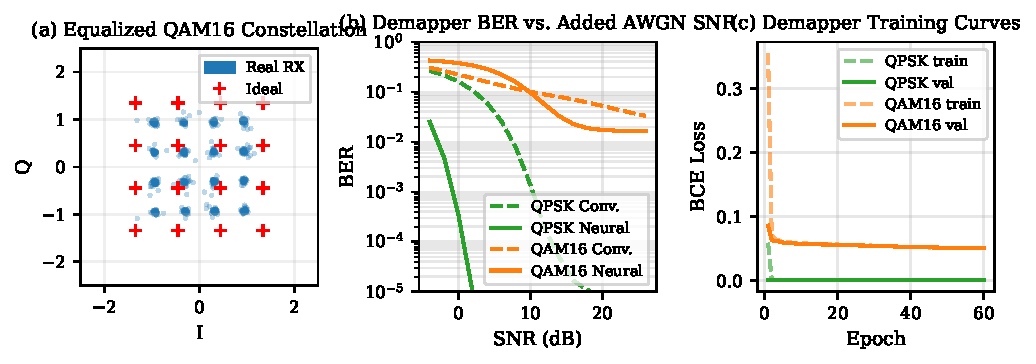
\includegraphics[width=\linewidth]{fig10_llr_demapper.pdf}
  \caption{(a) Equalized 16-QAM constellation from real hardware (blue
    scatter) overlaid on ideal grid points (red +);
    (b) BER vs.\ injected AWGN SNR for neural vs.\ conventional
    demapper (dashed = conventional, solid = neural);
    (c) training loss curves for QPSK and 16-QAM learned demappers.}
  \label{fig:llr}
\end{figure}

% ── VII. Related Work ─────────────────────────────────────────────────────────
\section{Related Work}
\label{sec:related}

Deep learning has been applied extensively to PHY tasks including
channel estimation~\cite{ye2018power}, signal detection~\cite{samuel2019deep},
and modulation classification~\cite{oshea2016convolutional}.
Most works use simulated channels or offline datasets.
\cite{o2017introduction} is an early exception advocating real-radio
benchmarking; our work extends this by integrating the data collection
and labelling pipeline into the receiver itself.

Schmidl-Cox synchronisation~\cite{schmidl1997robust} underpins our STF
design; the 4-pilot OFDM structure follows 802.11a conventions.
Neural gating for signal detection is related to learned preamble
detectors~\cite{peng2019deep}, but our approach differs by (a) running
before the demodulator, (b) using a pre-demod-only feature set, and
(c) coupling the gate to the data collection policy.

Automated radio dataset construction has been explored in
\cite{oshea2016convolutional,west2017deep} using channel emulators.
Our contribution is a real-hardware, fully automated pipeline with
three-tier negative-sample mining and iterative retraining.

% ── VIII. Conclusion ──────────────────────────────────────────────────────────
\section{Conclusion}
\label{sec:conclusion}

We presented \sys, a real-radio OFDM prototype that integrates the PHY
processing pipeline with automated dataset collection, annotation, and
iterative deep-learning model development.
The system demonstrates end-to-end operation: the PlutoSDR hardware link
delivers a raw BER\,=\,0 channel under good conditions, while the
automated sweep pipeline collected over 36{,}000 annotated captures
($>$30\,GB, 19{,}000\,+ NPZ archives) without any human labelling effort.
One complete improvement iteration is demonstrated: gate\_model\_v3,
trained from v3 QAM-16 hard-negative captures, was deployed live in the
v4 sweeps, achieving 96.9\% QPSK decode rate and 52.3\% QAM-16 decode
rate (up from 37.1\%), with the ADC-saturation signature (8.1\% at 60\,dB
vs.\ 65.6\% at 40\,dB) precisely confirming the target hard-negative regime.

Three documented lessons shape the practical design:
(1)~\emph{never include post-demodulation features in a pre-demodulation
classifier} — the feature-leakage pitfall that collapsed \gate{} v1;
(2)~\emph{hard negative mining from high-order modulation failures}
boosts gate ROC-AUC from 0.946 to 0.995 by focusing on the
ADC-saturation regime unique to 16-QAM;
(3)~\emph{end-to-end learning on raw preamble IQ} achieves equal
performance (AUC\,=\,0.996) without any hand-crafted features,
pointing toward a fully learned detection pipeline.

A learned soft demapper trained on the archived equalized symbols via
self-supervised labels demonstrates hardware-adaptive demodulation that
generalises to injected noise levels below the hardware noise floor.

The three-tier Mixture Logger, non-blocking NPZ archiving, and
self-reinforcing retraining loop constitute a reusable
hardware-in-the-loop deep-learning infrastructure for communications
research, reproducible with commodity SDR hardware.

% ── References ────────────────────────────────────────────────────────────────
\begin{thebibliography}{10}

\bibitem{o2017introduction}
T.~J. O'Shea and J.~Hoydis,
``An introduction to deep learning for the physical layer,''
\emph{IEEE Trans. Cognitive Commun. Netw.}, vol.~3, no.~4,
pp.~563--575, Dec. 2017.

\bibitem{dorner2018deep}
S.~D\"{o}rner, S.~Cammerer, J.~Hoydis, and S.~ten Brink,
``Deep learning based communication over the air,''
\emph{IEEE J. Sel. Topics Signal Process.}, vol.~12, no.~1,
pp.~132--143, Feb. 2018.

\bibitem{schmidl1997robust}
T.~M. Schmidl and D.~C. Cox,
``Robust frequency and timing synchronization for OFDM,''
\emph{IEEE Trans. Commun.}, vol.~45, no.~12, pp.~1613--1621, Dec. 1997.

\bibitem{ye2018power}
H.~Ye, G.~Y. Li, and B.-H. Juang,
``Power of deep learning for channel estimation and signal detection in
OFDM systems,''
\emph{IEEE Wireless Commun. Lett.}, vol.~7, no.~1, pp.~114--117, 2018.

\bibitem{samuel2019deep}
N.~Samuel, T.~Diskin, and A.~Wiesel,
``Learning to detect,''
\emph{IEEE Trans. Signal Process.}, vol.~67, no.~10,
pp.~2554--2564, May 2019.

\bibitem{oshea2016convolutional}
T.~J. O'Shea, J.~Corgan, and T.~C. Clancy,
``Convolutional radio modulation recognition networks,''
in \emph{Proc. Eng. Appl. Neural Netw.}, 2016, pp.~213--226.

\bibitem{peng2019deep}
S.~Peng, H.~Jiang, H.~Wang, H.~Alwageed, Y.~Zhou, M.~M. Sebdani,
and Y.-D. Yao,
``Modulation classification based on signal constellation diagrams and
deep learning,''
\emph{IEEE Trans. Neural Netw. Learn. Syst.}, vol.~30, no.~3,
pp.~718--727, Mar. 2019.

\bibitem{west2017deep}
N.~E. West and T.~J. O'Shea,
``Deep architectures for modulation recognition,''
in \emph{Proc. IEEE DySPAN}, 2017, pp.~1--6.

\end{thebibliography}

\end{document}
